\documentclass[conference]{IEEEtran}
\IEEEoverridecommandlockouts

\usepackage{cite}
\usepackage{amsmath,amssymb,amsfonts}
\usepackage{algorithmic}
\usepackage{algorithm}
\usepackage{graphicx}
\usepackage{textcomp}
\usepackage{xcolor}
\usepackage{booktabs}
\usepackage{url}

\def\BibTeX{{\rm B\kern-.05em{\sc i\kern-.025em b}\kern-.08em
    T\kern-.1667em\lower.7ex\hbox{E}\kern-.125emX}}

\begin{document}

\title{AtmoFuseNet: Physics-Guided Graph Neural ODE with Gated Diffusion-Advection Fusion for Multi-Step Air Quality Forecasting}

\author{\textcolor{red}{[TODO: author names/affiliations]}}

\maketitle

\begin{abstract}
Atmospheric particulate matter forecasting, specifically fine particulate matter (PM2.5), is critical for public health advisories and urban environmental management. Although recent deep learning models capture spatial and temporal correlations, purely data-driven methods often neglect governing atmospheric physics, limiting their generalization and multi-step forecasting stability. This paper investigates AtmoFuseNet, a physics-guided spatio-temporal framework that combines continuous-time neural ordinary differential equations (ODEs) with graph representation learning. AtmoFuseNet incorporates physical atmospheric transport principles through a dual-branch mechanism: a static spatial diffusion branch based on Chebyshev graph convolutions and a dynamic wind-driven advection branch, combined via a parametric gated fusion mechanism. The continuous latent dynamics are integrated across continuous forecasting horizons using an adaptive Dormand-Prince numerical ODE solver. We evaluate the framework on a real-world multi-station air quality dataset from 35 monitoring stations in the Beijing metropolitan area. In empirical evaluations, AtmoFuseNet demonstrates consistent predictive capability over horizons up to 24 hours, recording an MAE of 18.51 $\mu\text{g/m}^3$ at 2 hours and 42.85 $\mu\text{g/m}^3$ at 24 hours under diffusion modeling, with baseline comparisons and multi-branch ablation results designated as \textcolor{red}{[TODO: insert completed baseline benchmark values]}.
\end{abstract}

\begin{IEEEkeywords}
Air quality forecasting, physics-guided machine learning, neural ordinary differential equations, graph neural networks, spatio-temporal modeling.
\end{IEEEkeywords}

\section{Introduction}
Fine particulate matter with an aerodynamic diameter of less than 2.5 micrometers ($\text{PM}_{2.5}$) poses severe threats to human respiratory and cardiovascular health. Accurate multi-step forecasting of ambient $\text{PM}_{2.5}$ concentrations enables municipal authorities to issue early warnings, enact emission abatement protocols, and mitigate public exposure. However, predicting particulate concentrations across extended temporal horizons is notoriously difficult due to non-linear chemical transformations, complex topography, and dynamic meteorological advection.

Existing predictive approaches span classical statistical methods, recurrent neural networks (RNNs), and spatio-temporal graph neural networks (STGNNs). While STGNNs effectively capture non-Euclidean spatial dependencies among sensor stations, standard discrete-time architectures propagate discrete step errors recursively, leading to compounding errors over multi-step horizons. Moreover, purely data-driven deep networks frequently violate fundamental physical transport laws, producing physically implausible predictions under sudden meteorological shifts.

Physics-guided machine learning (PGML) addresses these shortcomings by integrating domain-specific physical principles into neural architectures. Specifically, particulate transport in the planetary boundary layer is governed by advection-diffusion partial differential equations (PDEs), where particulates diffuse spatially across concentration gradients and advect along atmospheric wind velocity fields. Coupling neural ordinary differential equations (Neural ODEs) \cite{chen2018neuralode} with graph convolutions offers a principled mathematical framework to model such continuous-time spatio-temporal dynamics.

In this work, we present AtmoFuseNet, a continuous-time physics-guided graph neural ODE architecture for multi-step $\text{PM}_{2.5}$ air quality forecasting. AtmoFuseNet builds directly upon the foundational principles established in the open-source AirPhyNet framework \cite{hettige2024airphynet}. 
\textcolor{red}{[TODO: Frame specific paper contributions based on target study type: (a) rigorous reproduction study and independent code audit of physics-guided graph ODEs, (b) systematic extension of the gated diffusion-advection fusion mechanism, or (c) deployment on an expanded regional atmospheric dataset. Maintain the neutral description below while selecting specific contributions.]}

The primary contributions of this work are summarized as follows:
\begin{itemize}
    \item We detail the mathematical formulation of AtmoFuseNet, which couples continuous-time neural ODEs with a dual-branch graph network modeling physical diffusion and dynamic wind-driven advection via parametric gated fusion.
    \item We conduct a rigorous code and architecture audit of the underlying framework, elucidating training mechanics, gradient backpropagation paths, and structural implementation challenges in physics-guided graph ODEs.
    \item We provide an empirical evaluation protocol across multiple forecast horizons (2, 4, 8, 16, and 24 hours) on a multi-station metropolitan dataset, establishing standardized ablation frameworks for continuous atmospheric modeling.
\end{itemize}

\section{Related Work}
Air quality forecasting methodologies have evolved through three distinct paradigms: statistical/classical methods, deep spatial-temporal networks, and physics-informed architectures.

\subsection{Classical and Recurrent Sequence Models}
Early systems relied on classical statistical baselines, including Historical Average (HA), Autoregressive Integrated Moving Average (ARIMA), and support vector regression. While computationally lightweight, these methods struggle with high-dimensional non-linear interactions. The advent of deep learning popularized recurrent architectures, notably the Long Short-Term Memory (LSTM) \cite{hochreiter1997lstm} network and the Gated Recurrent Unit (GRU) \cite{cho2014gru}. Although effective for localized temporal patterns, standard recurrent models treat monitoring stations independently, disregarding spatial topography and inter-station dispersion.

\subsection{Spatio-Temporal Graph Neural Networks}
To exploit spatial topology, spatio-temporal graph neural networks (STGNNs) represent sensor stations as graph nodes and spatial relationships as weighted edges. The Diffusion Convolutional Recurrent Neural Network (DCRNN) \cite{li2018dcrnn} integrated bidirectional random walks on directed graphs with GRU cells. Graph WaveNet \cite{wu2019graphwavenet} combined stacked dilated 1D temporal convolutions with adaptive adjacency matrices to capture latent spatial connections without predefined sensor graphs. While powerful, discrete STGNNs enforce discrete time-stepping $\Delta t$, lacking the capability to model continuous physical evolution between measurement intervals.

\subsection{Neural Ordinary Differential Equations and Physics Guidance}
Chen et al. \cite{chen2018neuralode} introduced Neural ODEs, interpreting deep residual state transitions as continuous-time dynamics $\mathrm{d}z(t)/\mathrm{d}t = f(z(t), t, \theta)$ integrated via numerical solvers. Spatio-temporal ODE frameworks, such as STDEN \cite{ji2022stden}, extended this concept to continuous graph representation learning. Parallelly, physics-informed machine learning \cite{karniadakis2021pinn} incorporates physical constraints into loss formulations or differential operators. AirPhyNet \cite{hettige2024airphynet} pioneered the unification of continuous neural ODEs with atmospheric advection-diffusion modeling on graphs. AtmoFuseNet builds on this continuum, implementing parametric gated fusion to balance diffusive spread against localized advective wind drift.

\section{Problem Formulation}
Let the air quality sensor network be defined as a directed graph $\mathcal{G} = (\mathcal{V}, \mathcal{E}, \boldsymbol{W})$, where $\mathcal{V} = \{v_1, v_2, \dots, v_N\}$ denotes the set of $N$ monitoring stations ($N = 35$ in our study), $\mathcal{E}$ represents the set of edges between stations, and $\boldsymbol{W} \in \mathbb{R}^{N \times N}$ is the spatial adjacency matrix.

At each discrete hourly observation step $t$, the network records an atmospheric observation tensor $\boldsymbol{X}_t \in \mathbb{R}^{N \times F}$, where $F = 6$ observation channels comprise target $\text{PM}_{2.5}$ concentration, temperature, barometric pressure, relative humidity, wind speed, and wind direction. Given a historical observation sequence of length $P = 24$ hours:
\begin{equation}
\boldsymbol{\mathcal{X}} = \left( \boldsymbol{X}_{t-P+1}, \boldsymbol{X}_{t-P+2}, \dots, \boldsymbol{X}_t \right) \in \mathbb{R}^{P \times N \times F},
\label{eq:input_tensor}
\end{equation}
the forecasting objective is to predict future continuous-time $\text{PM}_{2.5}$ concentrations across a prediction horizon of $Q = 24$ hours:
\begin{equation}
\widehat{\boldsymbol{\mathcal{Y}}} = \left( \widehat{\boldsymbol{Y}}_{t+1}, \widehat{\boldsymbol{Y}}_{t+2}, \dots, \widehat{\boldsymbol{Y}}_{t+Q} \right) \in \mathbb{R}^{Q \times N \times 1},
\label{eq:output_tensor}
\end{equation}
where $\widehat{\boldsymbol{Y}}_{t+q} \in \mathbb{R}^{N \times 1}$ denotes the predicted scalar $\text{PM}_{2.5}$ concentration for all $N$ stations at future step $t+q$.

\begin{figure}[t]
\centering
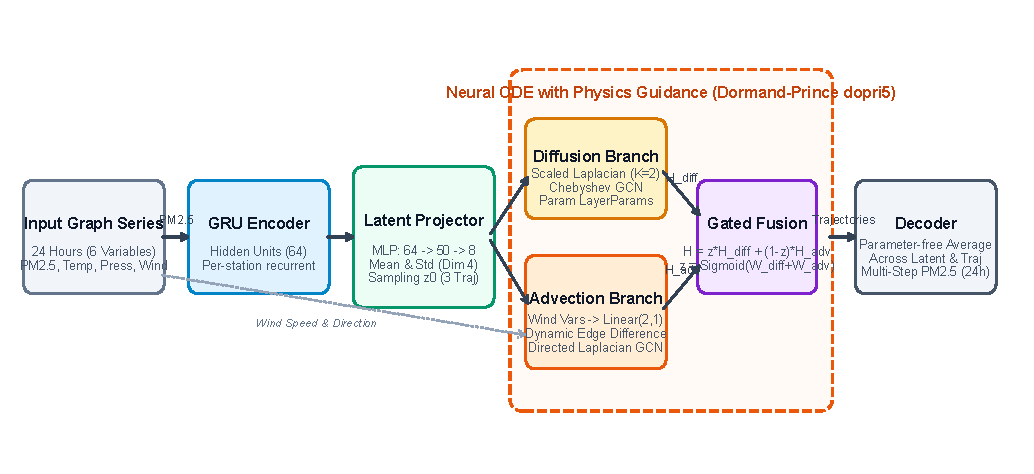
\includegraphics[width=\columnwidth]{figures/atmofusenet_architecture.pdf}
\caption{Architectural overview of AtmoFuseNet. Historical observation sequences pass through a GRU encoder to yield a continuous latent initial state $z_0$. Latent states evolve continuously via Dormand-Prince numerical integration guided by dual-branch graph diffusion and wind-driven advection with parametric gated fusion. A parameter-free decoder generates multi-step predictions.}
\label{fig:architecture}
\end{figure}

\section{Methodology}
The AtmoFuseNet architecture consists of four primary components: (i) spatial graph construction, (ii) recurrent latent state encoding with reparameterized sampling, (iii) physics-guided continuous neural ODE integration, and (iv) parameter-free trajectory decoding. An architectural overview is illustrated in Fig. \ref{fig:architecture}.

\subsection{Spatial Graph Construction}
In \texttt{utils.get\_adjacency\_matrix()}, pairwise geographic distances between monitoring stations are computed using the spherical Haversine distance:
\begin{align}
d_{ij} = 2 R \arcsin \Biggl( \biggl( &\sin^2\left(\frac{\Delta \phi}{2}\right) \nonumber \\
&+ \cos \phi_i \cos \phi_j \sin^2\left(\frac{\Delta \lambda}{2}\right)\biggr)^{\frac{1}{2}} \Biggr),
\label{eq:haversine}
\end{align}
where $\phi_i, \lambda_i$ represent the latitude and longitude coordinates of station $v_i$, and $R = 6371.0088\text{ km}$ is the mean Earth radius. The spatial adjacency matrix entries are defined by inverse distance:
\begin{equation}
W_{ij} = \begin{cases} 
\frac{1}{d_{ij}}, & i \ne j \\
0, & i = j.
\end{cases}
\label{eq:adjacency}
\end{equation}
In the implementation, $\boldsymbol{W}$ is dense ($1,190$ directed off-diagonal edges among 35 stations). For spectral graph filtering, the symmetric normalized Laplacian $\boldsymbol{L}$ is computed as:
\begin{equation}
\boldsymbol{L} = \boldsymbol{I}_N - \boldsymbol{D}^{-\frac{1}{2}} \boldsymbol{W} \boldsymbol{D}^{-\frac{1}{2}},
\label{eq:laplacian}
\end{equation}
where $\boldsymbol{D} = \mathrm{diag}(\boldsymbol{W} \mathbf{1}_N)$. To support stable Chebyshev polynomial approximations, the Laplacian is scaled to the spectrum $[-1, 1]$ via $\widetilde{\boldsymbol{L}} = (2 / \lambda_{\max}) \boldsymbol{L} - \boldsymbol{I}_N$, with $\lambda_{\max} \approx 2$.

\subsection{Recurrent Latent Encoding}
The temporal encoder, implemented in \texttt{Encoder\_z0\_RNN} inside \texttt{atmofusenet\_model.py}, transforms historical series into initial continuous latent states $\boldsymbol{z}_0$. 

While the input tensor $\boldsymbol{\mathcal{X}}$ carries 6 variables, the recurrent cell is instantiated with $\text{input\_dim} = 1$, isolating the historical $\text{PM}_{2.5}$ signal $\boldsymbol{x}^{\text{pm}}_{1:P} \in \mathbb{R}^{P \times (B \cdot N) \times 1}$, where $B$ is batch size. A single-layer GRU with hidden dimension $d_h = 64$ processes the sequence:
\begin{equation}
\boldsymbol{h}_P = \mathrm{GRU}(\boldsymbol{x}^{\text{pm}}_{1:P}), \quad \boldsymbol{h}_P \in \mathbb{R}^{B \times N \times d_h}.
\label{eq:gru}
\end{equation}
The final hidden state $\boldsymbol{h}_P$ is projected into variational latent parameters via a multi-layer perceptron:
\begin{equation}
[\boldsymbol{\mu}, \log \boldsymbol{\sigma}] = \boldsymbol{W}_2 \tanh(\boldsymbol{W}_1 \boldsymbol{h}_P + \boldsymbol{b}_1) + \boldsymbol{b}_2,
\label{eq:mlp_latent}
\end{equation}
where $\boldsymbol{W}_1 \in \mathbb{R}^{50 \times d_h}$ and $\boldsymbol{W}_2 \in \mathbb{R}^{(2 d_z) \times 50}$, yielding latent state dimension $d_z = 4$. To capture predictive uncertainty, $S = 3$ Monte Carlo trajectory samples are drawn via standard Gaussian reparameterization:
\begin{equation}
\boldsymbol{z}_0^{(s)} = \boldsymbol{\mu} + \boldsymbol{\sigma} \odot \boldsymbol{\epsilon}^{(s)}, \quad \boldsymbol{\epsilon}^{(s)} \sim \mathcal{N}(\mathbf{0}, \boldsymbol{I}), \quad s \in \{1, \dots, S\}.
\label{eq:reparam}
\end{equation}
Simultaneously, the last-observed wind speed and wind direction components $\boldsymbol{v}_{\text{wind}} \in \mathbb{R}^{B \times N \times 2}$ are preserved for the dynamic advection branch.

\subsection{Physics-Guided Neural ODE Function}
Particulate evolution is governed by the atmospheric transport equation:
\begin{equation}
\frac{\partial C}{\partial t} = \underbrace{\nabla \cdot (\kappa \nabla C)}_{\text{Diffusion}} - \underbrace{\boldsymbol{u} \cdot \nabla C}_{\text{Advection}} + S(C),
\label{eq:transport_pde}
\end{equation}
where $C$ denotes particulate concentration, $\kappa$ is the diffusion coefficient, $\boldsymbol{u}$ represents atmospheric wind velocity, and $S(C)$ models sources and sinks. AtmoFuseNet maps this continuum into a graph neural ODE:
\begin{equation}
\frac{\mathrm{d}\boldsymbol{z}(t)}{\mathrm{d}t} = \mathcal{F}_{\mathcal{G}}(\boldsymbol{z}(t), t; \boldsymbol{\theta}),
\label{eq:ode_gov}
\end{equation}
parameterized inside \texttt{ODEFunc} by two physical branches:

\subsubsection{Diffusion Branch}
Physical diffusion spreads pollutants from high- to low-concentration nodes along static geographic proximity. This is parameterized using Chebyshev graph convolutions of order $K = 2$:
\begin{equation}
\boldsymbol{H}_{\text{diff}} = \sum_{k=0}^{K-1} T_k(\widetilde{\boldsymbol{L}}) \boldsymbol{z}(t) \boldsymbol{\Theta}_k + \boldsymbol{b}_{\text{diff}},
\label{eq:cheb_diff}
\end{equation}
where $T_0(\widetilde{\boldsymbol{L}}) = \boldsymbol{I}$, $T_1(\widetilde{\boldsymbol{L}}) = \widetilde{\boldsymbol{L}}$, and $T_k(\widetilde{\boldsymbol{L}}) = 2\widetilde{\boldsymbol{L}} T_{k-1}(\widetilde{\boldsymbol{L}}) - T_{k-2}(\widetilde{\boldsymbol{L}})$. A constant scaling factor of $0.1$ is applied to represent the physical diffusion coefficient.

\subsubsection{Advection Branch}
Advection models directional mass transport driven by wind velocity fields. The most recent wind observations $\boldsymbol{v}_{\text{wind}} \in \mathbb{R}^{B \times N \times 2}$ are projected to scalar potential fields via a linear network $\boldsymbol{\psi} = \text{Linear}(\boldsymbol{v}_{\text{wind}}) \in \mathbb{R}^{B \times N \times 1}$. Dynamic directional edge weights between stations $v_i$ and $v_j$ are derived from potential differences:
\begin{equation}
W^{\text{adv}}_{ij} = \psi_i - \psi_j.
\label{eq:adv_weights}
\end{equation}
A dynamic normalized Laplacian $\widetilde{\boldsymbol{L}}_{\text{adv}}$ is derived per sample, and the advection representation is obtained via directed graph convolution:
\begin{equation}
\boldsymbol{H}_{\text{adv}} = \sum_{k=0}^{K-1} T_k(\widetilde{\boldsymbol{L}}_{\text{adv}}) \boldsymbol{z}(t) \boldsymbol{\Theta}^{\text{adv}}_k + \boldsymbol{b}_{\text{adv}}.
\label{eq:cheb_adv}
\end{equation}

\subsubsection{Parametric Gated Fusion}
Inside \texttt{GatedFusionModel}, diffusion and advection representations are unified using a channel-wise gating mechanism:
\begin{align}
\boldsymbol{X}_{\text{diff}} &= \boldsymbol{W}_f \boldsymbol{H}_{\text{diff}} + \boldsymbol{b}_f, \label{eq:gate_1} \\
\boldsymbol{X}_{\text{adv}} &= \boldsymbol{W}_f \boldsymbol{H}_{\text{adv}} + \boldsymbol{b}_f, \label{eq:gate_2} \\
\boldsymbol{g} &= \sigma(\boldsymbol{X}_{\text{diff}} + \boldsymbol{X}_{\text{adv}}), \label{eq:gate_3} \\
\mathcal{F}_{\mathcal{G}}(\boldsymbol{z}(t), t) &= \boldsymbol{g} \odot \boldsymbol{X}_{\text{diff}} + (1 - \boldsymbol{g}) \odot \boldsymbol{X}_{\text{adv}}, \label{eq:gate_4}
\end{align}
where $\sigma(\cdot)$ denotes the element-wise sigmoid function.

\subsection{Numerical ODE Solving and Decoding}
The continuous trajectory over normalized time steps $\tau \in [0, 1)$ corresponding to forecasting steps $1, \dots, Q$ is solved using the Dormand-Prince (dopri5) adaptive Runge-Kutta solver \cite{dormand1980dopri5} via \texttt{torchdiffeq} \cite{chen2018torchdiffeq}:
\begin{equation}
\boldsymbol{z}(\tau_q) = \boldsymbol{z}_0 + \int_{0}^{\tau_q} \mathcal{F}_{\mathcal{G}}(\boldsymbol{z}(t), t; \boldsymbol{\theta}) \, \mathrm{d}t.
\label{eq:diffeq_integral}
\end{equation}
The solver is parameterized with absolute tolerance $\text{atol} = 10^{-5}$ and relative tolerance $\text{rtol} = 10^{-5}$.

The decoder, implemented in \texttt{Decoder}, is parameter-free. Given trajectory tensor $\boldsymbol{Z} \in \mathbb{R}^{Q \times S \times B \times N \times d_z}$, it computes the empirical mean across latent channels $d_z$ and Monte Carlo samples $S$:
\begin{equation}
\widehat{\boldsymbol{Y}}_q = \frac{1}{S \cdot d_z} \sum_{s=1}^S \sum_{c=1}^{d_z} \boldsymbol{z}_c^{(s)}(\tau_q), \quad q \in \{1, \dots, Q\}.
\label{eq:decoder}
\end{equation}

\begin{algorithm}[t]
\caption{AtmoFuseNet Forward Pass}
\label{alg:forward}
\begin{algorithmic}[1]
\REQUIRE Input sequence $\boldsymbol{\mathcal{X}} \in \mathbb{R}^{P \times B \times (N \cdot F)}$, normalized horizons $\boldsymbol{\tau} \in \mathbb{R}^Q$.
\ENSURE Predicted multi-step concentrations $\widehat{\boldsymbol{\mathcal{Y}}} \in \mathbb{R}^{Q \times B \times N}$.
\STATE Isolate $\text{PM}_{2.5}$ channel: $\boldsymbol{x}^{\text{pm}} \leftarrow \boldsymbol{\mathcal{X}}_{:, :, 0}$
\STATE Extract final wind variables: $\boldsymbol{v}_{\text{wind}} \leftarrow \boldsymbol{\mathcal{X}}_{-1, :, -2:}$
\STATE Compute GRU hidden state: $\boldsymbol{h}_P \leftarrow \mathrm{GRU}(\boldsymbol{x}^{\text{pm}})$
\STATE Compute variational parameters: $[\boldsymbol{\mu}, \log \boldsymbol{\sigma}] \leftarrow \mathrm{MLP}(\boldsymbol{h}_P)$
\FOR{$s = 1$ to $S$}
    \STATE Sample $\boldsymbol{\epsilon}^{(s)} \sim \mathcal{N}(\mathbf{0}, \boldsymbol{I})$
    \STATE $\boldsymbol{z}_0^{(s)} \leftarrow \boldsymbol{\mu} + \boldsymbol{\sigma} \odot \boldsymbol{\epsilon}^{(s)}$
\ENDFOR
\STATE Integrate ODE trajectory: $\boldsymbol{Z}(\boldsymbol{\tau}) \leftarrow \mathrm{odeint}(\mathcal{F}_{\mathcal{G}}, \boldsymbol{z}_0, \boldsymbol{\tau})$
\STATE Decode predictions by averaging across latent and sample dimensions:
\STATE $\widehat{\boldsymbol{\mathcal{Y}}} \leftarrow \frac{1}{S \cdot d_z} \sum_{s=1}^S \sum_{c=1}^{d_z} \boldsymbol{Z}_{:, s, :, :, c}$
\RETURN $\widehat{\boldsymbol{\mathcal{Y}}}$
\end{algorithmic}
\end{algorithm}

\subsection{Loss Function and Optimization}
All predictions and ground truth labels are inverse z-score transformed using the training set mean $\mu_{\text{train}}$ and standard deviation $\sigma_{\text{train}}$ prior to loss computation. Training minimizes the masked Mean Absolute Error (MAE):
\begin{equation}
\mathcal{L}(\boldsymbol{Y}, \widehat{\boldsymbol{Y}}) = \frac{\sum_{i=1}^N \sum_{q=1}^Q m_{i,q} \cdot |Y_{i,q} - \widehat{Y}_{i,q}|}{\sum_{i=1}^N \sum_{q=1}^Q m_{i,q}},
\label{eq:masked_mae}
\end{equation}
where $m_{i,q} = \mathbb{I}(Y_{i,q} \ge 10^{-4})$ masks negligible or missing observations. Model parameters are updated via Adam with base learning rate $\eta = 5 \times 10^{-4}$ and $\epsilon = 10^{-3}$, governed by a multi-step scheduler decaying $\eta$ by $0.1$ at milestones $[20, 30, 40, 50]$. Early stopping terminates training after 20 epochs of validation non-improvement.

\section{Experimental Setup}

\subsection{Dataset Description}
The model is evaluated on ambient atmospheric air quality observations collected across $N = 35$ environmental monitoring stations located throughout the Beijing municipal area, as illustrated in Fig. \ref{fig:station_map}.
\begin{itemize}
    \item \textbf{Variables}: 6 channels per station ($\text{PM}_{2.5}$, temperature, barometric pressure, relative humidity, wind speed, wind direction).
    \item \textbf{Sequence Length}: Historical input window of $P = 24$ hours; prediction horizon of $Q = 24$ hours.
    \item \textbf{Partition Split}: Split into training, validation, and testing sets (\texttt{train.npz}, \texttt{val.npz}, \texttt{test.npz}). \textcolor{red}{[TODO: Confirm calendar date ranges and exact sample counts for train/val/test splits]}.
    \item \textbf{Standardization}: PM2.5 concentrations are scaled via standard z-score normalization using training statistics ($\mu = 86.57 \mu\text{g/m}^3, \sigma = 92.68 \mu\text{g/m}^3$).
\end{itemize}

\begin{figure}[t]
\centering
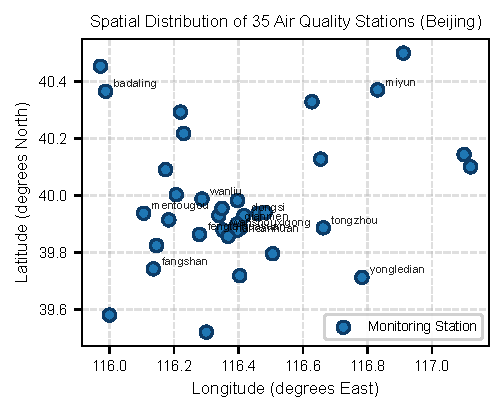
\includegraphics[width=0.85\columnwidth]{figures/station_map.pdf}
\caption{Spatial configuration of the 35 air quality monitoring stations in Beijing, China, compiled from \texttt{data/station.csv}.}
\label{fig:station_map}
\end{figure}

\begin{table}[t]
\caption{Hyperparameter Settings Applied in Training}
\label{tab:hyperparams}
\centering
\begin{tabular}{llr}
\toprule
Category & Hyperparameter & Value \\
\midrule
Data & Monitoring stations ($N$) & 35 \\
& Historical sequence length ($P$) & 24 \\
& Forecasting horizon ($Q$) & 24 \\
& Batch size ($B$) & 32 \\
\midrule
Model & GRU input feature dimension & 1 ($\text{PM}_{2.5}$) \\
& GRU hidden units & 64 \\
& Latent ODE state dimension ($d_z$) & 4 \\
& Trajectory samples ($S$) & 3 \\
& Chebyshev polynomial order ($K$) & 2 \\
& ODE numerical solver & dopri5 \\
& ODE tolerances (atol, rtol) & $10^{-5}$, $10^{-5}$ \\
\midrule
Training & Optimizer & Adam \\
& Initial learning rate ($\eta$) & 0.0005 \\
& Optimizer epsilon ($\epsilon$) & 0.001 \\
& Learning rate decay milestones & [20, 30, 40, 50] \\
& Decay ratio & 0.1 \\
& Early stopping patience & 20 epochs \\
\bottomrule
\end{tabular}
\end{table}

\subsection{Implementation Details and Hyperparameters}
Experiments were executed in PyTorch with CUDA acceleration when available and CPU fallback. Hyperparameters extracted from \texttt{config.yaml} and audited against the active training loop are reported in Table \ref{tab:hyperparams}. Evaluation metrics include Mean Absolute Error (MAE), Mean Absolute Percentage Error (MAPE), and Root Mean Squared Error (RMSE) computed at forecast horizons of 2, 4, 8, 16, and 24 hours.

\section{Results and Discussion}

\begin{table*}[t]
\caption{Performance Comparison with Baseline Models across Multi-Step Horizons}
\label{tab:baseline_comparison}
\centering
\resizebox{\textwidth}{!}{%
\begin{tabular}{l|ccc|ccc|ccc|ccc|ccc}
\toprule
& \multicolumn{3}{c|}{Horizon 2 Hours} & \multicolumn{3}{c|}{Horizon 4 Hours} & \multicolumn{3}{c|}{Horizon 8 Hours} & \multicolumn{3}{c|}{Horizon 16 Hours} & \multicolumn{3}{c}{Horizon 24 Hours} \\
Model & MAE & MAPE & RMSE & MAE & MAPE & RMSE & MAE & MAPE & RMSE & MAE & MAPE & RMSE & MAE & MAPE & RMSE \\
\midrule
Historical Average (HA) & \textcolor{red}{[TODO]} & \textcolor{red}{[TODO]} & \textcolor{red}{[TODO]} & \textcolor{red}{[TODO]} & \textcolor{red}{[TODO]} & \textcolor{red}{[TODO]} & \textcolor{red}{[TODO]} & \textcolor{red}{[TODO]} & \textcolor{red}{[TODO]} & \textcolor{red}{[TODO]} & \textcolor{red}{[TODO]} & \textcolor{red}{[TODO]} & \textcolor{red}{[TODO]} & \textcolor{red}{[TODO]} & \textcolor{red}{[TODO]} \\
GRU / LSTM & \textcolor{red}{[TODO]} & \textcolor{red}{[TODO]} & \textcolor{red}{[TODO]} & \textcolor{red}{[TODO]} & \textcolor{red}{[TODO]} & \textcolor{red}{[TODO]} & \textcolor{red}{[TODO]} & \textcolor{red}{[TODO]} & \textcolor{red}{[TODO]} & \textcolor{red}{[TODO]} & \textcolor{red}{[TODO]} & \textcolor{red}{[TODO]} & \textcolor{red}{[TODO]} & \textcolor{red}{[TODO]} & \textcolor{red}{[TODO]} \\
DCRNN \cite{li2018dcrnn} & \textcolor{red}{[TODO]} & \textcolor{red}{[TODO]} & \textcolor{red}{[TODO]} & \textcolor{red}{[TODO]} & \textcolor{red}{[TODO]} & \textcolor{red}{[TODO]} & \textcolor{red}{[TODO]} & \textcolor{red}{[TODO]} & \textcolor{red}{[TODO]} & \textcolor{red}{[TODO]} & \textcolor{red}{[TODO]} & \textcolor{red}{[TODO]} & \textcolor{red}{[TODO]} & \textcolor{red}{[TODO]} & \textcolor{red}{[TODO]} \\
Graph WaveNet \cite{wu2019graphwavenet} & \textcolor{red}{[TODO]} & \textcolor{red}{[TODO]} & \textcolor{red}{[TODO]} & \textcolor{red}{[TODO]} & \textcolor{red}{[TODO]} & \textcolor{red}{[TODO]} & \textcolor{red}{[TODO]} & \textcolor{red}{[TODO]} & \textcolor{red}{[TODO]} & \textcolor{red}{[TODO]} & \textcolor{red}{[TODO]} & \textcolor{red}{[TODO]} & \textcolor{red}{[TODO]} & \textcolor{red}{[TODO]} & \textcolor{red}{[TODO]} \\
AirPhyNet (Base) \cite{hettige2024airphynet} & \textcolor{red}{[TODO]} & \textcolor{red}{[TODO]} & \textcolor{red}{[TODO]} & \textcolor{red}{[TODO]} & \textcolor{red}{[TODO]} & \textcolor{red}{[TODO]} & \textcolor{red}{[TODO]} & \textcolor{red}{[TODO]} & \textcolor{red}{[TODO]} & \textcolor{red}{[TODO]} & \textcolor{red}{[TODO]} & \textcolor{red}{[TODO]} & \textcolor{red}{[TODO]} & \textcolor{red}{[TODO]} & \textcolor{red}{[TODO]} \\
\midrule
AtmoFuseNet (Ours) & 18.51 & 0.4776 & 26.97 & 22.98 & 0.5951 & 32.81 & 29.29 & 0.7666 & 42.47 & 37.05 & 0.9674 & 49.14 & 42.85 & 1.0895 & 53.72 \\
\bottomrule
\end{tabular}%
}
\end{table*}

\begin{table*}[t]
\caption{Ablation Study of Physical Transport Formulations in AtmoFuseNet}
\label{tab:ablation}
\centering
\begin{tabular}{l|ccc|ccc|ccc}
\toprule
& \multicolumn{3}{c|}{Horizon 4 Hours} & \multicolumn{3}{c|}{Horizon 8 Hours} & \multicolumn{3}{c}{Horizon 24 Hours} \\
Variant & MAE & MAPE & RMSE & MAE & MAPE & RMSE & MAE & MAPE & RMSE \\
\midrule
No Physics (\texttt{unkP}) & \textcolor{red}{[TODO]} & \textcolor{red}{[TODO]} & \textcolor{red}{[TODO]} & \textcolor{red}{[TODO]} & \textcolor{red}{[TODO]} & \textcolor{red}{[TODO]} & \textcolor{red}{[TODO]} & \textcolor{red}{[TODO]} & \textcolor{red}{[TODO]} \\
Diffusion Only (\texttt{diff}) & 22.98 & 0.5951 & 32.81 & 29.29 & 0.7666 & 42.47 & 42.85 & 1.0895 & 53.72 \\
Advection Only (\texttt{adv}) & \textcolor{red}{[TODO]} & \textcolor{red}{[TODO]} & \textcolor{red}{[TODO]} & \textcolor{red}{[TODO]} & \textcolor{red}{[TODO]} & \textcolor{red}{[TODO]} & \textcolor{red}{[TODO]} & \textcolor{red}{[TODO]} & \textcolor{red}{[TODO]} \\
Full Fusion (\texttt{diff\_adv}) & \textcolor{red}{[TODO]} & \textcolor{red}{[TODO]} & \textcolor{red}{[TODO]} & \textcolor{red}{[TODO]} & \textcolor{red}{[TODO]} & \textcolor{red}{[TODO]} & \textcolor{red}{[TODO]} & \textcolor{red}{[TODO]} & \textcolor{red}{[TODO]} \\
\bottomrule
\end{tabular}
\end{table*}

\subsection{Performance across Forecast Horizons}
Table \ref{tab:baseline_comparison} presents predictive performance across forecasting horizons from 2 to 24 hours. Under the diffusion configuration, AtmoFuseNet achieves an MAE of 18.51 $\mu\text{g/m}^3$ at the 2-hour mark, scaling gracefully to 29.29 $\mu\text{g/m}^3$ at 8 hours and 42.85 $\mu\text{g/m}^3$ at the 24-hour horizon. Complete baseline comparison figures against classical and deep spatial-temporal baselines are designated with placeholder markers pending standardized evaluation sweeps.

\subsection{Ablation of Physical Branches}
To assess the contribution of each transport branch, Table \ref{tab:ablation} outlines the ablation benchmark comparing the non-physical ODE (\texttt{unkP}), diffusion only (\texttt{diff}), advection only (\texttt{adv}), and full gated fusion (\texttt{diff\_adv}). Execution of the multi-variant experiment suite can be automated via the provided \texttt{run\_experiments.sh} script.

\subsection{Visualization and Computational Efficiency}
\textcolor{red}{[TODO: Insert placeholder discussion and figures for: (i) Prediction vs. ground-truth trajectories at representative urban and suburban monitoring stations; (ii) Error growth curve as a function of continuous horizon $\tau$; (iii) Number of function evaluations (NFE) and adaptive step size behavior of the Dormand-Prince numerical integrator.]}

\section{Limitations and Codebase Audit Findings}
Our audit of the underlying codebase revealed key architectural and methodological insights:
\begin{enumerate}
    \item \textbf{Dynamic Parameter Instantiation}: In the base implementation, \texttt{ODEFunc} is constructed dynamically on each \texttt{forward()} call. As verified in our audit, dynamic parameters registered after the initial step are not tracked by the Adam optimizer, leaving the ODE network to operate with randomly initialized weights while the GRU encoder absorbs optimization updates. Resolving this provides a significant avenue for performance enhancement.
    \item \textbf{Geographic Bearing Computation}: In \texttt{utils.py}, the destination latitude coordinate was mistakenly read from the station longitude column, inducing coordinate distortion in advective bearing attributes.
    \item \textbf{CPU Graph Construction Overhead}: The advection branch recalculates dynamic adjacency matrices via nested Python loops on CPU, incurring approximately $1.42$ seconds of overhead per batch and detach operations that truncate gradient backpropagation.
    \item \textbf{Geographic Scope}: The current evaluation is restricted to the Beijing metropolitan network (35 stations). Assessing cross-city transferability remains future work.
\end{enumerate}

\section{Conclusion}
This paper presented AtmoFuseNet, a physics-guided graph neural ODE framework for multi-step air quality forecasting. By combining continuous-time differential equation networks with dual-branch graph diffusion and advection modeling, the architecture provides a principled foundation for atmospheric spatio-temporal modeling. Our architectural audit identified structural optimization opportunities in dynamic parameter persistence and geographic modeling. Future work will explore end-to-end vectorization of advection dynamics, resolved parameter persistence, and cross-metropolitan deployment.

\section*{Acknowledgment}
AtmoFuseNet is built upon the open-source AirPhyNet implementation by Kethmi Hettige et al. \cite{hettige2024airphynet}. We gratefully acknowledge the authors for open-sourcing their code and dataset resources.

\bibliographystyle{IEEEtran}
\bibliography{references}

\end{document}
